 \documentclass{llncs}

\usepackage[utf8x]{inputenc}
\usepackage{graphicx}
\usepackage{url}
\usepackage{listings}
%\usepackage[table]{xcolor}

\lstset{
  basicstyle=\scriptsize
}

\title{Linked Open Data as the fuel for Smarter Cities}

\author{Mikel Emaldi, Jon Lázaro, Oscar Peña, Diego López-de-Ipiña, Sacha Vanhecke}

\begin{document}
    \maketitle

    \abstract{In the last decade big efforts have been carried out in order to move towards the Smart City concept, from both the academic and industrial points of view, encouraging researchers and data stakeholders to find new solutions on how to cope with the huge amount of generated data.

Open Data has arisen as a way to share data in order to be consumed freely without restrictions from copyright, patents or other mechanisms of control. Nowadays Open Data is an achievable concept thanks to the World Wide Web, and has been re-defined for its application in different domains.

Regarding public administrations, the concept of Open Government has found an ally in Open Data concepts, defending citizens' right to access data, documentation and proceedings of the governments.

We propose the use of Linked Open Data, a set of best practices to publish data on the Web proposed by the W3C, in a new data life-cycle management model, allowing governments and individuals to handle better their data, easing the consumption by anybody, including both companies and third parties interested in the exploitation of the data, and citizens as end users receiving relevant curated information and reports about their city.

In summary, Linked Open Data uses the previous Openness concepts to evolve from an infrastructure thought for humans, to an architecture for the automatic consumption of big amounts of data, providing relevant and high quality data to end users with low maintenance costs. Smart data can now be achievable in smart cities.}

    \section{Introduction}

% Authors provide an ample introduction on the problem being addressed, 
% issues and challenges, motivating thus the chapter

Data management is becoming one of the greatest challenges of the $21^{st}$ century. Regarding urban growth, experts predict that global urban population will double by the year 2050, meaning that nearly 70\% of the whole planet's inhabitants will be living in a major town or city.

This prediction arises the need to deal with the huge amounts of data generated by cities, enabling the possibility to manage their resources in an efficient way. The \textit{Smart Data} term has been coined to address the data that makes itself understandable, by extracting relevant information and insights from big data and presenting the conclusions as human-friendly visualizations.

The problems of managing data are moving to a new level. It's not only a matter of caring about \textit{more} data, but how we can use it efficiently in our processes. It's about how we can deal with increasing volumes of data (from standalone databases to real \textit{Big Data}) and integrate them to our advantage, making it useful and digestible in order to make better decisions.

In the last few years, the \textit{Smart city} concept has been adopted to refer to those cities aware of their citizens' life quality, worried about the efficiency and trustworthiness of the services provided by governing entities and businesses.

Smart data can help cities reach a \textit{Smart City} status, analysing the generated data streams and providing useful information to their users: citizens, council managers, third parties, etc.

Although, efficient data lifecycle management processes need to be adopted as best practices, avoiding to convert input data in non-sense noise that can not be used to improve council's services.

Thus, our approach relies is based on an actual review of the state of the art regarding data lifecycle management, proposing our own model as a more refined approach to the existing ones. We also encourage the adoption of Linked Open Data principles to publish both the whole generated data and the processed data, in order to allow further research on the area by third parties and the development of new business models relying on public access data.
    
    \section{Background and definitions}
\label{subsec:background}

As envisaged by Sir Tim Berners-Lee, the Web is moving from a interlinked documents space to a global information one, where both documents and data are linked: The Semantic Web \cite{berners2001semantic}.

Linked Data is a set of best practices to publish data on the Web in a machine-readable way, with a explicitly defined semantic meaning, linked to other datasets and allowed to be searched for \cite{bizer2009linked}.

In 2006, Sir Tim Berners-Lee described a set of principles to publish Linked Data on the Web:

\begin{enumerate}
  \item Use URIs as names for things
  \item Use HTTP URIs so that people can look up those names
  \item When someone looks up a URI, provide useful information, using the standard (RDF, SPARQL)
  \item Include links to other URIs, so that they can discover more things \\[\baselineskip]
\end{enumerate} 

Later, in 2010, he established a five-star rating system to encourage people and governments to publish high-quality Linked Open Data: 

\begin{tabular}{ l p{0.75\linewidth} }
  $\star$ & Available on the web (whatever format) but with an \textbf{open licence}, to be Open Data \\
  $\star$ $\star$ & Available as machine-readable structured data (e.g. excel instead of image scan of a table) \\
  $\star$ $\star$ $\star$ & as (2) plus non-propietary format (e.g. CSV instead of excel) \\
  $\star$ $\star$ $\star$ $\star$ & All the above plus: Use open standards from W3C (RDF and SPARQL) to identify things, so that people can point at your stuff \\
  $\star$ $\star$ $\star$ $\star$ $\star$ & All the above plus: Link your data to other people's data to provide context \\[\baselineskip]
\end{tabular}

Following these recommendations, data publishers can move towards a new data-powered space, in which data scientists and application developers can research on new uses for Linked Open Data.

    \section{Data Life Cycle}

Throughout the literature, a variety of different definitions of data life cycle models can be found. Although they have been developed for different actuation domains, we describe here some of them which we think that can be applied for generic data, independently of its original domain.

\subsection{Data Documentation Initiative}

The first model to be analysed is the model proposed by Data Documentation Initiative (DDI). The DDI introduced a Combined Life Cycle Model for data managing \cite{data_documentation_initiative_overview_2008}. As Figure \ref{fig:ddi} shows, this model has eight elements or steps which can be summarized as follows, according to \cite{ball_review_2012}:

\begin{itemize}
    \item \textbf{Study concept.} At this stage, apart from choosing the research question and the methodology for collecting the data, also plans the processing and analysis of data to answer the question.
    \item \textbf{Data collection.} This model proposes different methods to collect data, like surveys, health records, statistics or Web-based collections.
    \item \textbf{Data processing.} At this stage, the collected data is processed to answer the proposed research question. The data may be recorded both machine-readable and human-readable form.
    \item \textbf{Data archiving.} Both data and metadata should be archived to ensure long-term access to them, ensuring the confidentiality.
    \item \textbf{Data distribution.} This stage involves the different ways which the data are distributed and questions related to terms of use of the data or citation of the original sources. 
    \item \textbf{Data discovery.} The data may be published in different manners, through publications, web-indexes, etc.
    \item \textbf{Data analysis.} The data can be used by others to achieve different goals.
    \item \textbf{Repurposing.} The data can be used outside of their original framework, restructuring them or combining with different data.
\end{itemize}

%TODO: Vectorialize
\begin{figure}
    \center
    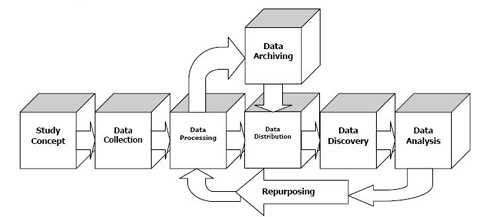
\includegraphics[width=\textwidth]{img/data_lifecycle/what-is-ddi-diagram.jpg}
    \caption{Combined Life Cycle Model (ownership: DDI Alliance).}
    \label{fig:ddi}
\end{figure}

%\footnotetext{\url{http://www.ddialliance.org/}}

\subsection{Australian National Data Service}

In late 2007 the Australian National Data Service (ANDS) was founded with the target of creating a national data management environment. ANDS established a set of verbs, denominated Data Sharing Verbs that describe the entire life cycle of the data \cite{burton_designing_2009}:

\begin{itemize}
    \item \textbf{Create.} \textit{Create} (or \textit{collect} for disciplines with an observational focus) is about the kinds of metadata that could be collected and the tools for fulfill this collection task.
    \item \textbf{Store.} This \textit{Sharing Verb} remarks the need for stable and web-accessible storage, taking care about the appropriate storing of data.
    \item \textbf{Describe.} The more information is inside the storage, more difficult is its discovery, access and exploit. Annotating the data with the proper metadata solves this issue.
    \item \textbf{Identify.} The application of this verb implies the proper identification of each data resource, assigning a persistent identifier to each of them.
    \item \textbf{Register.} This Verb pertains to registering the descriptions of the different data collections with one or more public catalogues.
    \item \textbf{Discover.} To improve the data-reusing, ANDS suggests to enable different discovery services.
    \item \textbf{Access.} To guarantee the appropriate access to data, ANDS suggests to provide a suitable search engine to retrieve these data. If the data is not electronically available, ANDS recommends to provide contact details to get the data in conventional forms.
    \item \textbf{Exploit.} \textit{Exploit}, the final Data Verb, involves the tools, methodologies and support actions to enable reutilisation of data.
\end{itemize}

\subsection{Ecoinformatics data life cycle}

Michener and Jones define in \cite{michener_ecoinformatics:_2012} the concept of ``ecoinformatics'': \textit{a framework that enables scientists to generate new knowledge through innovative tools and approaches for discovering, managing, integrating, analysing, visualizing and preserving relevant biological, environmental, and socioeconomic data and information.} To manage these data, the following data life cycle has been defined, as can be seen at Figure \ref{fig:ecoinformatics}:
\begin{itemize}
    \item \textbf{Plan.} This step involves the confection of a data management planning.
    \item \textbf{Collect.} This step consider both manual (hand-written data sheets) and automatic (sensor networks) data-collection methods.
    \item \textbf{Assure.} Quality assurance and quality control (QA/QC), an issue which in previously mentioned models is not taken into account, refers to developing methods to guarantee the integrity of the data. Quality assurance also can consists of defining standards for formats, codes, measurement units, metadata, etc.
    \item \textbf{Describe.} As other data life cycle models, this model remarks the value of the metadata to answer to questions about \textit{who, when, where, how} and \textit{why}.
    \item \textbf{Preserve.} Data preservation implies the storage of the data and metadata, ensuring that these data can be verified, replicated and actively curated over time.
    \item \textbf{Discover.} The authors describe the data discover as \textit{one of the greatest challenges}, as many data are not immediately available because there are stored in individual laptops. The main challenges to publish the data in a proper way are related about the creation of catalogues and indexes, and about the implementation of the proper search engines.
    \item \textbf{Integrate.} Integrating data from different and heterogeneous sources can become into a difficult task because it requires \textit{understanding methodological differences, transforming data into a common representation, and manually converting and recording data to compatible semantics before analysis can begin}.
    \item \textbf{Analyze.} As well as the importance of a clear analysis, this models remarks the importance of documenting this analysis with sufficient detail to enable its reproduction in different research frameworks.
\end{itemize}

\begin{figure}
    \center
    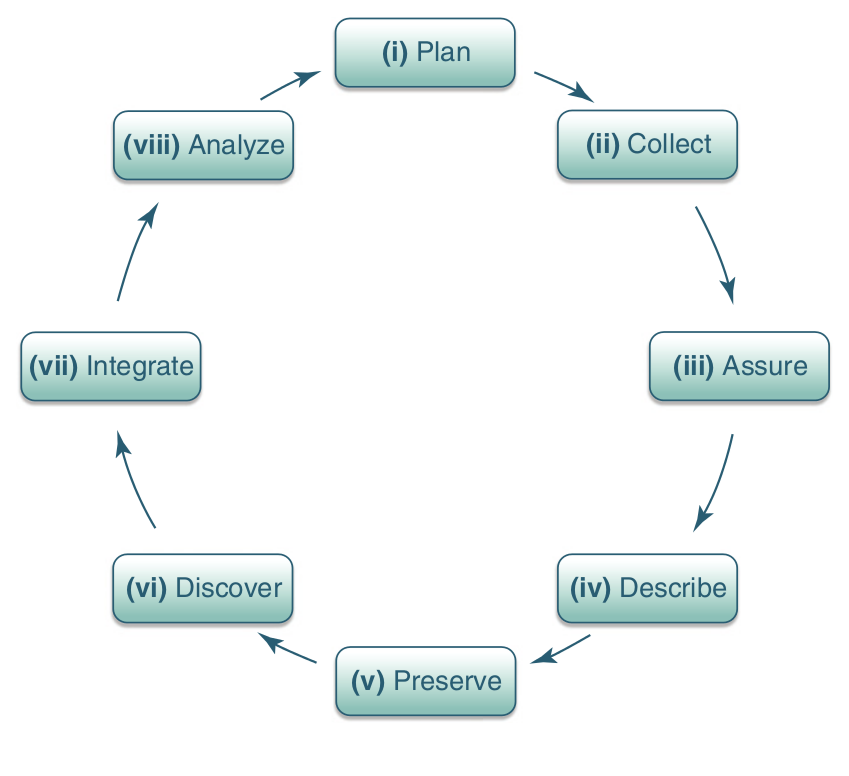
\includegraphics[scale=0.3]{img/data_lifecycle/ecoinformatics.png}
    \caption{Data life cycle in ecoinformatics. Taken from \cite{michener_ecoinformatics:_2012}.}
    \label{fig:ecoinformatics}
\end{figure}

\subsection{UK Data Archive}

The last analyzed data life cycle model, is the one proposed by UK Data Archive\footnote{\url{http://www.data-archive.ac.uk/create-manage/life-cycle}}. This model is oriented to help researchers to publish their data in a manner which allows other researchers continuing their work independently. In Figure \ref{fig:uk-data-archive}, we can observe the following stages:
\begin{itemize}
    \item \textbf{Creating data.} Creating the data involves the design of the research question, planning data management and their sharing. If we want to reuse existing data, we have to locate existing data and collect these data. As well as the data is new or is an existing data, at this stage the metadata has to be created.
    \item \textbf{Processing data.} Like in other models, at this stage the data is translated, checked, validated and cleaned. In the case of the confidential data, they have to be ``anonymized''. The UK Data Archive recommends to create the metadata at this stage too.
    \item \textbf{Analysing data.} At this stage the data are interpreted and derived into visualizations or reports. In addition, the data are prepared for preservation, as can be seen at following stage.
    \item \textbf{Preserving data.} To preserve the data properly, they are migrated to the best format and stored in a suitable medium. In addition to the previously created metadata, the creating, processing, analysis and preserving process are documented.
    \item \textbf{Giving access to data.} Once the data is stored, we have to distribute our data. This distribution of the data may involve controlling the access to them and establish a sharing license.
    \item \textbf{Re-using data.} At last, the data can be re-used enabling new research topics.
\end{itemize}

\begin{figure}
    \center
    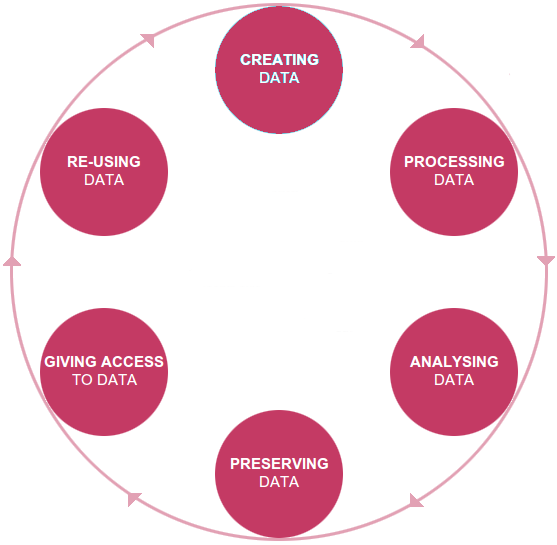
\includegraphics[scale=0.4]{img/data_lifecycle/uk-data-archive.png}
    \caption{Data life cycle proposed by UK Data Archive.}
    \label{fig:uk-data-archive}
\end{figure}

\subsection{A common data life cycle for smart cities}

Based on these data life cycle models, we proposed a common data life cycle for managing data into smart cities. As can be seen at Figure \ref{fig:model}, the different stages of mentioned models have been aggregated, forming our proposed model.
%\begin{table}
%    \centering
%    \begin{tabular}{|l|l|l|l|l|}
%        \hline
%        \textbf{DDI} & \textbf{ANDS} & \textbf{Ecoinformatics} & \textbf{UK Data Archive} & \\
%        \hline \hline
%        \rowcolor [gray]{.9} Study  concept & Create & Plan & Create & \\
%        \cellcolor [gray]{.9} Collect & \cellcolor [gray]{.8} Store & \cellcolor [gray]{.9} Collect & Process & \\
%        Process & Describe & Assure & Analyze & \\
%        Archive & Identify & Describe & Preserve & \\
%        Distribute & Register & Preserve & Access & \\
%        Discovery & Discover & Discover & Re-use & \\
%        Analysis & Access & Integrate & &  \\
%        Repurposing & Exploit & Analyze & & \\
%        \hline
%   \end{tabular}
%\end{table}

\begin{figure}
    \center
    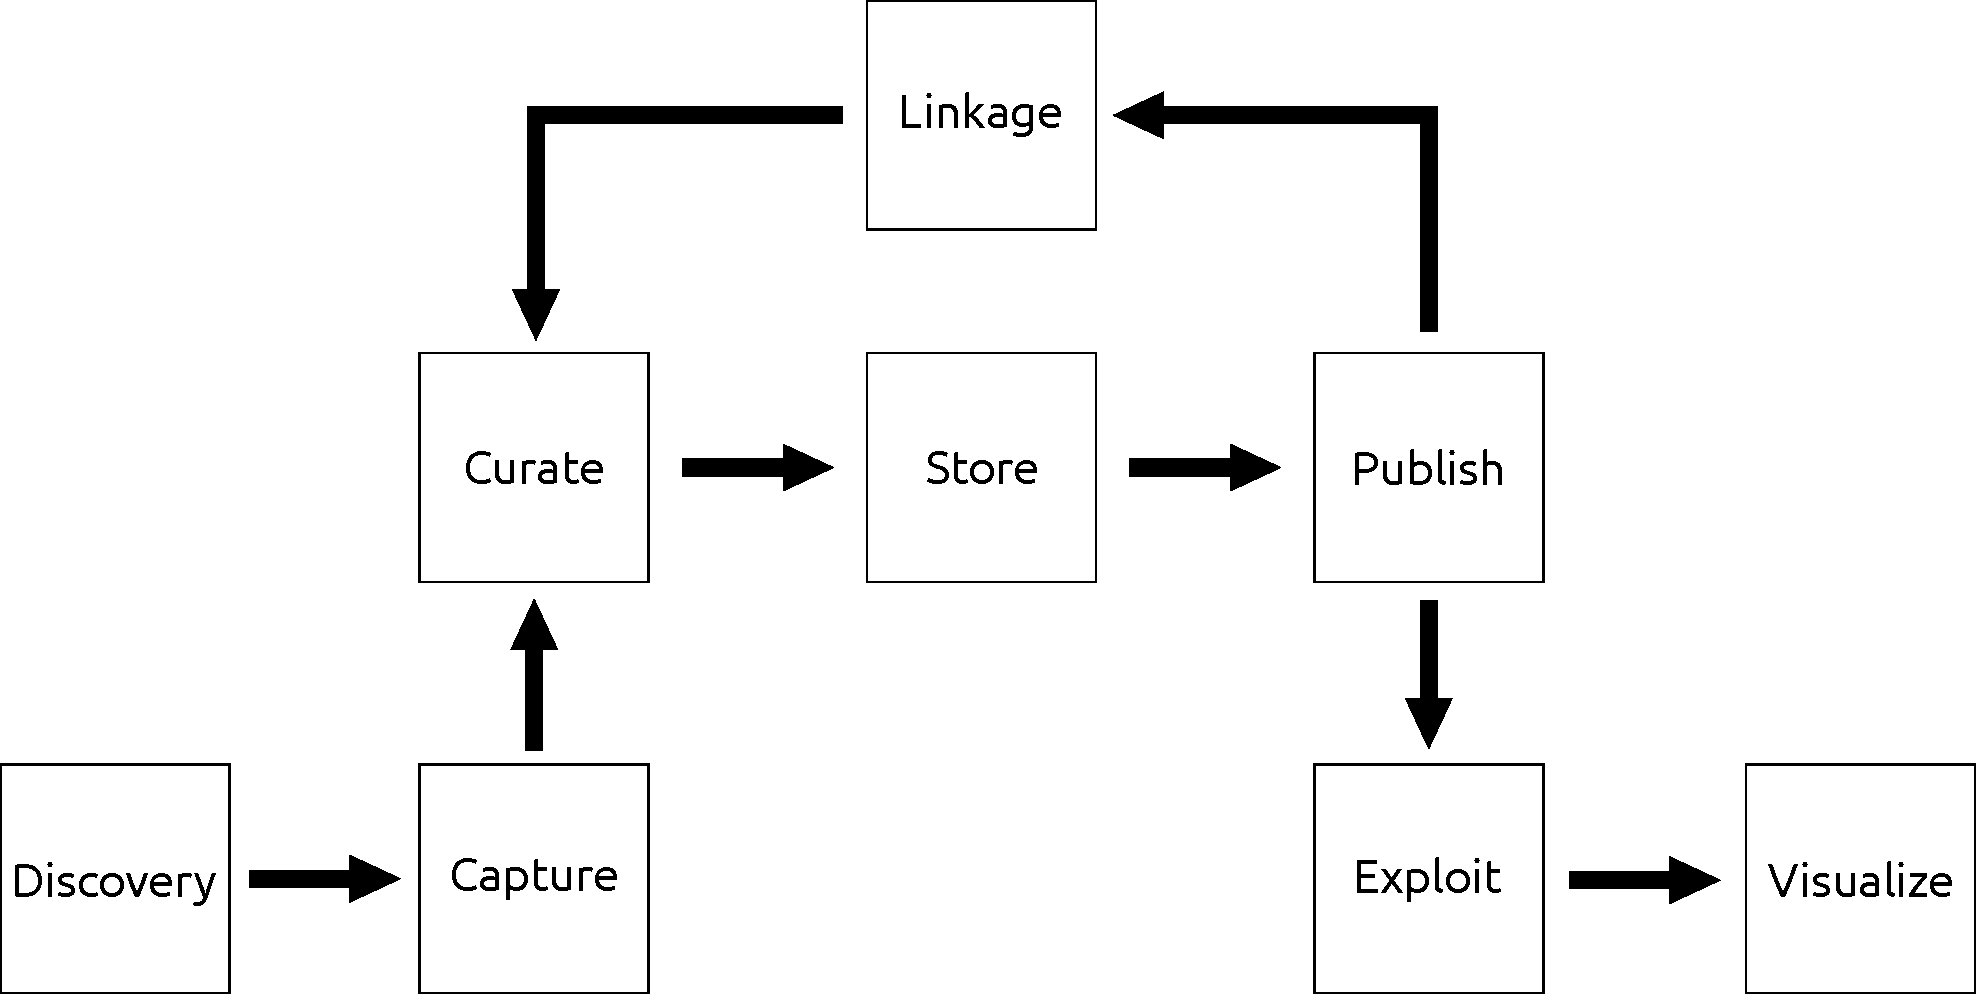
\includegraphics[width=\linewidth]{img/data_lifecycle/model.pdf}
    \caption{Proposed model.}
    \label{fig:model}
\end{figure}

The different stages of this model, which are going to be explained widely in following sections, are:
\begin{itemize}
    \item \textbf{Capture.} The first step of our model consists on capturing the data. In a smart city there are a lot of alternatives to capture data, like sensors, data published by public administration, social networks or in more traditional way like surveys.
    \item \textbf{Process.} Once the required data is captured, they are prepared to store, allowing proper methods to explore them. This processing involves the refining, cleaning, formatting and transformation of the data.
    \item \textbf{Store.} The storage of data is, probably, the most delicate action in the life cycle. Above the storage are build all the analysis tools and is the ``final endpoint'' when someone requests our data. A suitable storage should have indexing, replication, distribution and backup capabilities, among other things.
    \item \textbf{Publish.} Most of mentioned models 
    \item \textbf{Analyze.}
    \item \textbf{Visualize.}
    \item \textbf{Discovery.}
\end{itemize}



    \section{Identified challenges}

Taking into consideration the large amounts of data present at smart cities, data management's complexity can be described in terms of:
\begin{itemize}
	\item Volume
	\item Variety
	\item Veracity
	\item Velocity
\end{itemize}

This four variables can also be found in \textit{Big Data}-related articles (also known as the \textit{Big Data's Vs}) \cite{zikopoulos2011understanding,russom2011big}, so it is not surprising at all that smart cities are going to deal with Big Data problems in the near future (if they are not dealing with them right now).

Data scientist need to take into account these variables, which could overlap in certain enviroments. Should this happen, each scenario will determine the most relevant factors of the process, generating unwelcome drawbacks on the other ones.

\subsection{Volume}

The high amount of data generated and used by cities nowadays needs to be properly analysed, processed, stored and eventually accessible. This means conventional IT structures need to evolve, enabling scalable storage technologies, distributed querying approaches and massively parallel processing algorithms and architectures.

There is a growing trend which defends that the minimum amount of data should be stored and analysed without significantly affecting the overall knowledge that could be extracted from the whole dataset. Based on \textit{Pareto's Principle} (also known as the 80-20 rule), the idea is to focus on a 20\% of the data to be able to extract up to the 80\% of knowledge within it. Even being a solid research challenge in Big Data, there are ocassions where we can not discard data from being stored or analysed (e.g., sensor data about monitoring a building can be used temporally, while patient monitoring data should be kept for historical records).

% Apache Hadoop, MapReduce, No-SQL...

However, big amounts of data should not be seen as a drawback attached to smart cities. The larger the datasets, the better analysis algorithms can perform, so deeper insights and conclusions should be expected as an outcome. These could ease the decission making stage.

As management consultant Peter Drucker once said: \textit{``If you can not measure it, you can not manage it''}, thus leaving no way to improve it either. This adage manifests that should you want to take care of some process, but you are not able to measure it or you can not access the data, you will not be able to manage that process. That being said, the higher amounts of data available, the greater the opportunities of obtaining useful knowledge will become.

\subsection{Variety}

Data is rarely found in a perfectly ordered and ready for processing format. Data scientists are used to work with diverse sources, which seldom fall into neat relational structures: embedded sensor data, documents, media content, social data, etc. As can be seen at section \ref{sec:capture} there are many different sources where data can come from in a smart city. Despite of presented data cycle can be applied for all kind of data, the different steps of the cycle have to be planificated, avoiding the overloading of implemented system. For example, data from social media talking about an emergency situation may be prioritised over the rest of the data, to allow Emergency Response Teams (ERTs) react as soon as possible.

Moreover, different data sources can describe the same real world entities in such different ways, finding conflicting information, different data-types, etc. Taking care of how data sources describe their contents will lead to an easier integration step, lowering development, analytics and maintenance costs over time.

\subsection{Veracity}

There is also an increasing concern on data trustworthiness. Different data sources can have meaningful differences in terms of quality, coverage, accuracy, timeliness and consistency of the provided data. In fact, \cite{xian_truth_2013} conclude that redundancy, consistency, correctness and copying between sources are the most recurrent issues we have to deal with when we try to find trustworthy information from a wide variety of heterogeneous sources.

As pointed out by \cite{buneman2013data}, \textit{data provenance is fundamental to understanding data quality}. They also highlight that established information storage systems may not be adecuate to keep semantic sense of data.

Several efforts are trying to convert existing data in high quality data, providing an extra confidence layer in which data analysts can rely. In a previous research \cite{emalditrust}, we introduced a provenance data model to be used in user-generated Linked Data datasets, which follow W3C's PROV-O ontology\footnote{http://www.w3.org/TR/prov-o/}. Some other researchs as \cite{hartig_using_2009} or \cite{bizer_quality_2009} also provide some mechanisms to measure the quality and trust in Linked Data.

\subsection{Velocity}

Finally, we must assume that data generation is experiencing an exponential growth. That forces our IT structure to not only tackle with volume issues, but with high processing rates. A widely spread concept among data businesses is that sometimes you can not rely on five-minute-old data for your business logic.

That is why \textit{streaming data} has moved from academic fields to industry to solve velocity problems. There are two main reasons to consider streaming processing:
\begin{itemize}
	\item Sometimes, input data is too fast to store in their entirety without rocketing costs.
	% At the extreme end of the scale, the Large Hadron Collider at CERN generates so much data that scientists must discard the overwhelming majority of it — hoping hard they’ve not thrown away anything usefu
	\item If applications mandate immediate response to the data, batch processes are not suitable. Due to the rise of smartphone applications, this trend is increasingly becoming a common scenario.
\end{itemize}


    \section{Open Linked data as a viable approach}
    
    \section{Introduction}

    \section{Lessons learned}

    \section{Further research}    

    \bibliographystyle{splncs}

    \bibliography{LOD_smart_cities}
    
    \section{Acronyms and terms}
    CSV     Comma Separated Values
    RDF     Resource Description Framework
    JSON    JavaScript Object Notation
    XML     eXtensible Markup Language
    LOD     Linked Open Data
    RDFa    Resource Description Framework in Attributes
    NLP     Natural Language Processing
    NER     Named Entity Recognition
    API     Application Programming Interface
    REST    REpresentational State Transfer
    SOAP    Simple Object Access Protocol
    WMS     Web Map Service
    RSS     Really Simple Syndication
    SPARQL  SPARQL Protocol and RDF Query Language
    POI     Point Of Interest
    URI     Uniform Resource Identifier
    KML     Keyhole Markup Language
    HTML    HyperText Markup Language
    HTTP    HyperText Transfer Protocol
    N3      Notation3
    JS      JavaScript
    TSV     Tab Separated Values
    SQL     Structured Query Language
    OWL     Web Ontology Language
    W3C     World Wide Web Consortium


\end{document}
